\documentclass[a4paper,11pt] {article}
\usepackage[english]{babel}

\usepackage{graphicx}
\usepackage{url}
\usepackage{amsmath}
\usepackage{caption}
\usepackage{subcaption}
\usepackage{natbib}
\usepackage{hyperref}
\usepackage[usenames,dvipsnames]{color}
\setlength{\parindent}{0 cm}
%%\usepackage{algorithmic}

% Title Page
\title{Shiny latex for SNE}
\author{
Leendert van Duijn\\
Esan Wit\\
MORE NAMES, alphabetical order\\}

\begin{document}
\maketitle
\newpage


\section{XML and XHTML}

\subsection{W3C Procedure for Recommendation}

The W3C procedure for recommendation is defined as follows: a working group creates a \textit{Working Draft} (which indicates the work in progress). This draft is refined to a \textit{Candidate Recommendation}. The \textit{Candidate Recommendation} is further refined to become a \textit{Proposed Recommendation}. A committee decides on whether or not a \textit{Proposed Recommendation} becomes a \textit{W3C Recommendation}. In between the stages there are rounds for feedback in which people from the community/industry are invited to criticize and help improve the document. This process is represented by image ~\ref{fig:RecommendationProcedure} below.

\vspace{10pt}

\begin{figure}[here]
	\centering
	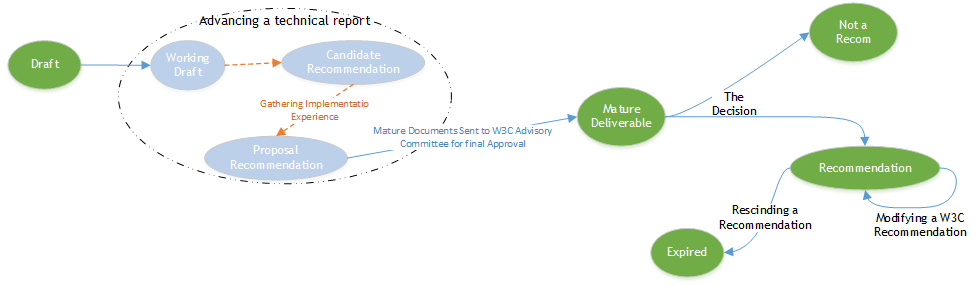
\includegraphics[width=1.0\textwidth]{images/w3c.png}
	\caption{An overview of the W3C Recommendation procedure. Image by Azad Kamali.}
	\label{fig:RecommendationProcedure}
\end{figure}

\subsection{IBM Technical Series}

For this assignment we had to watch three videos that can be found on YouTube:
\begin{itemize}
\item An Introduction to XML: The Basics \citep{ibmtechnicalpart1}
\item An Introduction to XML: XML and Web 2.0 \citep{ibmtechnicalpart2}
\item An Introduction to XML: Managing XML Data \citep{ibmtechnicalpart3}
\end{itemize}


We extracted the following insights from the videos about XML, of which the advantages can be found in table ~\ref{tab:XmlProsCons}. 
\begin{itemize}
\item
XML has a widespread usage everywhere in the industry and is a fully defined, open standard.
\item
It can be used as a meta language (a language describing the language itself).
XML enables easy sharing data between applications, independent of platform or software.
\item
RSS and ATOM allow to syndicate content to users, ATOM features reusable elements while RSS doesn't.
\item
AJAX allows the creation of dynamic web applications.
\item
RDF is the key-language in semantic web development and is XML-based. It describes resources.
\item
XML allows semi-structured or unstructured data, handles nested and complex data, and it's extensible
\item
XQuery and XPath allow to search XML data for specific fields, structures or information
\item
XSLT specifies how to transform XML documents into other XML documents (e.g. applying stylesheet to render XML in browser)
\end{itemize}

\paragraph{Short overview of advantages and disadvantages}
\mbox{}

\begin{table}[h]
\begin{tabular}{|l|l|}
\hline
	\textbf{\color{OliveGreen}Advantages} & \textbf{\color{Maroon}Disadvantages} \\
	\hline
	Widespread usage & Larger size XML records \\
	Platform independent & Implementation cost \\
	Allows for (un)structured data & Higher complexity for retrieval and storage \\
	Self-definable language & \\
\hline
\end{tabular}
\caption{The advantages and disadvantages of XML}
\label{tab:XmlProsCons}
\end{table}



%\documentclass[titlepage; draft]{report}
%	\author{A. ~Kamali, C.V. ~Bockhaven, E. Wit, L.V. Duijn}
%	\title{Further Reading \newline XML and XSLT concepts}
%	\date{\today}
%       \usepackage[usenames,dvi,svgames]{xcolor}
%	\usepackage{hyperref}

%\begin{document}
\section{Further Reading, XML and XSLT concepts}
\label{sect:azad}
\subsection{Transforming XML with XSLT}
	I found the following points in the \href{http://oreilly.com/catalog/orxmlapp/chapter/ch07.pdf}{Transforming XML with XSLT} interesting:
        \begin{itemize}
		\item When processing a document of XML, only a single matched template is used to process the current node.
		\item If a stylesheet uses only the root template, then it can optionally use the simple form stylesheet syntax that allows \verb~<xsl:stylesheet>~ and \verb~<xsl:template match="/">~ to be left out.
		\item It is possible to use multiple templates rather than s single root template.
        \item We can reuse the previously built templates by using \verb~<xsl:import mode>~.
		\item It is possible to use a sort of regular expression for matching rules.
		\item When you create a template, in addition to the match pattern, it can also have a mode attribute that assigns a name to the special mode in which you want to invoke the template.
		\item When applying multiple rules to one object, the most specific one wins.
		\item The basic scheme for determining which templates are more specific than others is as follows, ordered by ascending specificity:
		\begin{itemize} 
		    \item The generic pattern: \verb|*| 
		    \item Element name: \verb|SOMETHING| or \verb|xyz:SOMETHING|
		    \item Element path: \verb|SOMETHING/SOMETHINGELSE|
		    \item Element with matching predicate: \verb|SOMETHING[predicate]|
	    \end{itemize}
		\item All XSLT transformations process the source node tree to produce a tree of result nodes. If multiple transformations are being applied in sequence by your application, the result tree of one transformation becomes the source tree of the next transformation in sequence. When no more transformations need to be done, the final tree of result nodes needs to be written out as a stream of characters again. This process is called serializing the result tree.
		\item XSLT 1.0 supports three different output methods:
		    \begin{itemize}
            \item \verb~<xsl:output method=~{\color{red}\verb|"xml"|}\verb|/>|
		    \item \verb~<xsl:output method=~{\color{red}\verb|"html"|}\verb|/>|
		    \item \verb~<xsl:output method=~{\color{red}\verb|"text"|}\verb|/>|
	        \end{itemize}
        \end{itemize}
        
\subsection{Group Discussion Result}
Key point to the XSLT parsing is the XPath pattern matching system used to find and match source blocks with the templates. XSLT is modular and can be extended; when using multiple XSLT templates the template with a \verb|"match"| that is more specific then others is used to parse the source node. Templates with a higher specificity take precedence over less specific templates. 
	
E.g. \textcolor{red}{match="ROW"} has a lower specificity than "\textcolor{green}{match=ROW[ $SAL > 2000$ ]}" as such if "\textcolor{green}{match=ROW[ $SAL > 2000$ ]}" is applicable the template which matches merely "\textcolor{blue}{ROW}" is ignored;


This is different to the process of CSS; in CSS if multiple patterns match an element all rules that are defined for those patterns are applied to the element. If multiple of the applied CSS rules define the same properties the more specific rule overwrites the properties set by less specific rules. But non overridden properties are inherited from which ever rule defined them. In XSLT only the most specific template is used and less specific templates are not inherited;
	

XPath has support for certain mathematical operations. E.g. doing something special for each 5th row or special handling in case some input value is odd or even;
	

XSLT transformations can be chained. That is to say if multiple transformations are being applied in sequence of each other then the node tree which is the output of one transformation is used as the input of another transformation. This process is called serializing;
	

While making a stylesheet in order to make it easier to extend or edit your templates, one can make use of multiple templates rather than a single rooted template stylesheet.



\section{Auto-Tools}
\label{sect:esan}
\subsection{Introduction to the Autotools}
Introduction to the Autotools is a series of tutorial videos made by David A. Wheeler\cite{wheeler2012autopart1,wheeler2012autopart2,wheeler2012autopart3}.
Autotools is a collection of various tools designed to make the use of compiling source, and Make in particular, easier~\citep{wheeler2012autopart1}. Autotools can help creating platform independent sources~\citep{wheeler2012autopart1}. AutoMake, part of Autotools,  assists in solving dependencies of source files. It also supports the use of nested structures without the user having to create complicated makefiles~\cite{wheeler2012autopart2}. Autotools can be used to help cross-compilation on platforms~\citep{wheeler2012autopart2}. Autotools are bundled with methods to resolve and locate dependencies on a system.
Autotools supports the recursive make paradigm (although this should not be used, see \ref{sec:recursivemake})~\citep{wheeler2012autopart3}. It's advisable to prefer a large Makefile.am as opposed to a recursive build structure~\citep{miller1998recursive,wheeler2012autopart3}.

\subsection{Recursive Make Considered Harmful}
\label{sec:recursivemake}
Peter Miller wrote an article about the problems he noticed in the usage of the Make\cite{miller1998recursive}. Most notably the problems that originate from the Recursive Make paradigm.
Image~\ref{fig:peter_miller}\footnote{Source: \url{http://miller.emu.id.au/pmiller/}} shows him over the years.
\begin{figure} \centering
\captionsetup[subfigure]{labelformat=empty}
\begin{subfigure}{0.19\textwidth}

\includegraphics[width=\textwidth]{images/peter_miller_2009.jpg}
\caption{2009}
\end{subfigure}
\begin{subfigure}{0.19\textwidth}
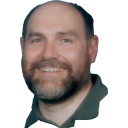
\includegraphics[width=\textwidth]{images/peter_miller_2003.png}
\caption{2003}
\end{subfigure}
\begin{subfigure}{0.19\textwidth}

\includegraphics[width=\textwidth]{images/peter_miller_1993.png}
\caption{1993}
\end{subfigure}
\begin{subfigure}{0.19\textwidth}

\includegraphics[width=\textwidth]{images/peter_miller_1981.png}
\caption{1981}
\end{subfigure}
\begin{subfigure}{0.19\textwidth}
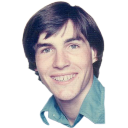
\includegraphics[width=\textwidth]{images/peter_miller_1975.png}
\caption{1975}
\end{subfigure}
\caption{Peter Miller over time}
\label{fig:peter_miller}
\end{figure}

The author describes several problems with recursive make and attributes these to make not being allowed to do it's work. Make resolves dependencies to determine what requires rebuilding and what doesn't. By the principles of recursive make this becomes impossible. Instead the author propagates the use of full project makefiles of a modular format. A user must then rebuild the entire project. This allows make to properly analyze the DAG for dependencies and determining which parts need to be updates.

The indexing cost of this is negligible when compared to the cost of over-building or rebuilding in order to prevent bugs and race conditions. This cost becomes even more negligible when the user takes into account the time saved with debugging. The recursive make paradigm is prone to several bugs and race-conditions. By removing recursive make from the equation time can be saved during development. E.g. time spend debugging the system as opposed to debugging the code.

The full project make also allows make to make full use of the option of parallel building. Because the entire DAG is available make can work on both ends simultaneously, with recursive make this is impossible because make is not aware of the greater scope of the dependencies.

\subsubsection{Present Day}
A lot of the reasons and arguments in favor of recursive makes are no longer applicable on current computers. Memory has become cheap and processing power too. With current design philosophies going towards greater parallelism it seems that the argument to allow make a full DAG are still applicable. The assumed un-manageability of big makefiles is stopped by the appearance of build tools which automate the process.




\section{Git and SVN}
\label{sect:leen}
\subsection{The polite programmer presents - Torvalds Vs the world of CVS}

\[
Git >  Mercurial > tar+patches > SVN > CVS
\label{math:linus-svn}
\]

Linus T. preferred source management methods are shown in relation \ref{math:linus-svn}.


\subsubsection{History, Bitkeeper}
An early scm, decent but why settle for less than perfect.
Git's flow is partially based on Bitkeeper but this was commercially distributed system which people did not like and could not even try to improve.

\subsubsection{Future, what features would a replacement have?}

\begin{enumerate}
  \item What goes in, comes out. Undetected corruption is not an option.
  \item Performance, if it takes too much time\ldots
  \item Merging easy, Branching is trivial. Merging should be easy.
  \item Diff, to show what and how much changed. But why only on files?
\end{enumerate}

\subsubsection{A distributed system}
What are possible motives for switching to a distributed system,
\begin{itemize}
 \item Centralized collaboration is hard due to branch cost, more accuratly merging branches.
 \item You dont\'t want a central location waiting to fail or be compromized.
 \item You don\'t want any single point of failure.
 \item You can work offline for longer periods of time.
 \item By distributing you have a crude form of backup as all copies can be used equally.
\end{itemize}

However, there are some properties a distributed system has which reduce the fun of building, using and maintaining it,
for example branching is required for any (offline) use. While the branching can
be rather cheap in terms of storage and computational requirements, the demand
for constant merging will require special care and introduce overhead in using
the system.


Using a distributed system you can benefit from a Trust network, by modelling
the repositories to be compatible you can easilly incorperate/pull code and patches
from those peers you trust, and by extension and smart merging, the peers they
trust. Each person can determine who has access to their own repository by means
of their own choice. A use case for this would be a realease team that can read
from a developers repository\footnote{but not write if they choose to} and
carefully test all changes they introduce into a 'verified' release grade
repository.

A team of developers, one of potentially many, can share their branches and
code without continously running into conflicts with other teams. Therefore enabling them to
develop complex experimental features collaboratively, while maintaining a stable codebase for
other teams who might work on their possibly related or even conflicting features.


A decent distributed code management system will allow a user to track the source and history of code, features and bugs.
By making sure a full history is available you can enjoy the power of quality reviews, or audits should someone expect foul play.


\subsubsection{The powers of Git}

\begin{itemize}
\item
Even if you don't care about Git and just adore CVS\footnote{Do not let L. Torvalds know this, for your own sake}
you can use Git just for merging, then put it all back in CVS.

\item
Git makes merging easier than the competition by automating what it can.

\item
Merging can be delegated to the best knowing party, in the case of a conflict the person who caused it will know best what to do.

\item
You dont need to see or share all existing branches, a developer work in a private experimental branch and push it out when done or decent.

\item
Branch names need not be unique across the globe so you can use natural names

\item
A 'super' project can contain references to multiple projects which can be shared, much like libraries of code.

\item
Git checksums everything, cryptographically secure, this to ensure the data you put in you also get out. It makes it harder to sabotage the history with nasty suprises.

\item
Trust your data to be valid, Git does all it can to detect corruption for you.

\item Trust the data even from a shaky source, as long as you have the checksum from another more reliable source.


\item
Git can track full history of changes, however if you really need to you can rewrite it, but you can't really hide the act.

\item 
Tracks history regardless of the files the content lives in, tracking history even if you move a piece of text arround.

\end{itemize}


\subsection{Hg Vs Git}
\label{sect:rebase}

%Figure of a mercurry blob vs an idiot
\begin{figure}[h]

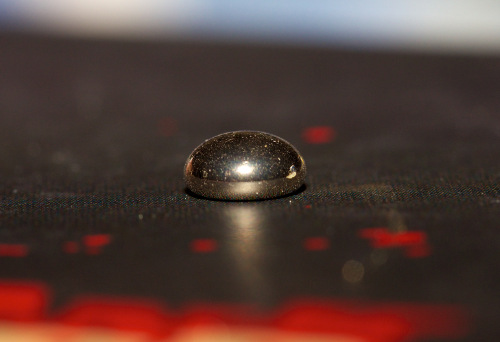
\includegraphics[width=\textwidth]{images/hg_blob_small.jpg}

\caption{Hg Blob, the metal}
\label{fig:hgblob}
\end{figure}

\textcolor{red}{Due to the nature of Mercury it would be dangerous to confuse the metal with the sofware, so illustrated in Figure \ref{fig:hgblob} is the dangerous metal, courtesy of Flickr\footnote{http://www.flickr.com/photos/hyper7/9530010713/, Creative Commons license}. Do not try to use any object like the one shown for version management of any code. You have been warned.}



When comparing Mercurial\footnote{Also known as Hg} with Git you can run into these statement, each relevant to selecting the system suited for you.
\begin{itemize}
\item
Hg history is sacred, you cannot change it.

\item
Git lets you rebase/change/destroy history 'easilly' if you explicitly instruct it to.

\item
Git does not really cater to SVN users, by design.

\item
There are plugins for both, with Hg having a tad more windows fiendly software, and Linux being the most efficient platform for Git.
If you use Eclipse just ignore the operating system, it has plugins for everything and anything.

\item
Hg cares about windows, which could be usefull when you run into a bug or want the last bit of performance you want.
Git can be run on windows at a small performance reduction when compared to Linux, but Git is more pleasant in a Linux environment.

\item
Hg might be more backwards compatible\footnote{Wikipdia style, Citation needed}, though we do have this on authority.

\item
Hg can support shell written extensions using alliasses, allowing core features to be accessed. This is a powerfull way to write plugins to extend the power of Hg.

\item
There are always options to buy commercial support for Hg.
Though Git will also have it's share of knowledgable consultants\footnote{Citition desired}.

\item
Hosting a git or Hg server can be done or done for you easilly at affordable fees.

\end{itemize}


Why could you choose Git as the best system for You?
\begin{enumerate}
\item
Things in git are immutable, being able to revert changes and undo mistakes is a useful safety net.

\item
Git history is safe and stored indefinately, unless you go to the trouble of telling Git to like in Section \ref{sect:rebase}
Rewriting history can be done in both Hg and Git, the Git way of doing so being quite powerful and once you know how, easier.

\item
Bragging rights, just because \textit{Branch} sounds cooler than \textit{bookmark}, and is actually a \textcolor{red}{core} feature.

\item
Git allows partial files to be committed, leaving some changes local if wanted (Such as a 'comment to self, spellcheck my name').
This still holds even for larger files, where it becomes much more useful.

\item
\large{\textit{git blame -C -s}}
Track ownership/history even if you move a feature or bug from \textcolor{green}{a.file} to \textcolor{blue}{b.file}.


\end{enumerate}


\subsubsection{A simple comparisson of VCS's}
There is always one rule to manage by;
Do not anger the programmer, choose the right DVCS

\begin{tabular}{|l|c|c|c|c|}
\hline
Feature             & CVS & SVN & Git & Hg\\
\hline
Mature              & +++ & ++  &  +  & + \\
Track moved content &  -  &  -  & +++ & + \\ %?hg svn
Atomical operations &  -  &  +  &  +  & + \\ 
Branching possible  &  +  &  +  &  +  & + \\
Branching pleasant  &  -  &  -  & +++ & + \\
P2P                 &  -  &  -  & +++ & ++\\ %? hg
Speed               &  -  &  -  & +++ & - \\
Offline history     &  -  &  -  &  +  & + \\
Windows compatible  &  +  &  +  &  +  &+++\\
Learning curve      &  +  &  +  &  -  & + \\
Documentation       &  +  &  +  &  +  & + \\ %? they are all documented, howto'ized etc.
2 parent merge      &  -  &  -  &  +  & - \\
Extensions          &  -  &  -  &  -  & + \\
Core power          &  -  &  -  &  +  & - \\
Small hosting cost  & low & low & low &low\\
Huge hosting cost   &High &High &low&low\\
\hline
\end{tabular}


Of course, learning to use any new system is bound to slow down progress for a while, so why not consider 
keeping the system that has been in place for a while now? Are you running into any problems? Changing VCS
will manage cause at least some problems.



\appendix

\bibliographystyle{unsrt}
\bibliography{freading.bib}

\end{document}
